\documentclass{article}

\usepackage{fullpage} % Makes the margins smaller
\usepackage{amsfonts,amsmath,amssymb} % Various math commands
\usepackage{graphicx} % To include pictures
\usepackage{bm} % To include code with \VerbatimInput
\usepackage{hyperref}
\usepackage{amsmath}
\usepackage{url}
\usepackage{graphicx}
\usepackage{tabularx}
\usepackage{filecontents}
\usepackage{tikz}
\usepackage{float}

\title{In-Class Kaggle Competition Writeup}
\author{Darien Zhang} % Make sure to change this!!!
\date{} % This omits the date, which we don't need

% This is the end of the document's preamble
\begin{document}
\maketitle

\noindent
1 Exploratory Analysis\\

\noindent
There are much more categorical variables than continuous variables. Since this will be a regression challenge, it may be better if I first transform the categorical variables to numbers and dig into the correlations and distribution of the continuous variables. \\

\noindent
Here is the correlation plot of all variables and continuous variables. \\

\begin{figure}[h]
\centerline{\begin{tabular}{cc}
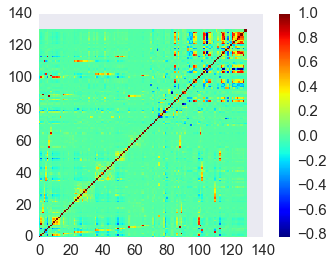
\includegraphics[width=0.2\textwidth]{correlation_all.png} &
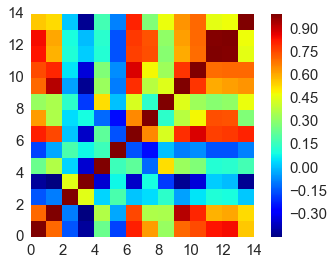
\includegraphics[width=0.2\textwidth]{correlation_conti.png}
\end{tabular}}
\caption{The left shows correlation among all variables. The right shows correlation among all continuous variables}
\label{fig:wall}
\end{figure}

\noindent
Here is the boxplots of the continuous variables.

\begin{figure}[H]
\centerline{\begin{tabular}{cc}
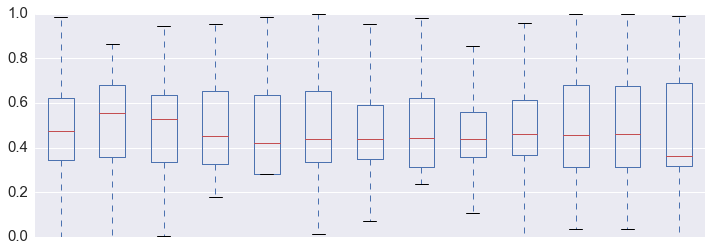
\includegraphics[width=0.5\textwidth]{boxplot.png}
\end{tabular}}
\caption{Boxplots of continuous variables}
\end{figure}

\noindent
Since there are some strong correlations detected and considering we have quite a lot of variables, one thing we can do is to conduct PCA for possible future usage. To do this, I also need to scale the data features.\\

\noindent
From the EDA we can get some basic idea of the data and some data preprocessing can be conducted. The detailed steps of data preprocessing can be found in the code. The most important thing I have done is turning categorical variables to numerical and scaled the data for future usage (like training neural networks). Since from the box plot we can see that there is not much outliers, we do not need robust scaler when scaling data. Furthermore, We could see some strong correlations among continous variable. This is why I try Ridge regression and use principle components as inputs in some models.\\


\noindent
2 Models \\

\noindent
Since this is a regression problem, I first tried on the multivariate linear regression as the baseline model. Based on this. I also tried Principle Component regression and Ridge regression.  However, the predictive accuracy is not very ideal. Thus, to depict such complicated non-linear realtionship and make predictions, I would like to use Random Forest and Neural Network as two of the algorithms to try on for this competition. We can import RandomForestRegressor from sklearn.ensemble, which will provide a good random forest regressor (not classifier) suitable for this problem. One big reason for choosing Random forest is that there are fewer hyperparameters to tune (Basically number of trees and max depth) and it is a ensemble method which can be powerful.  Theoretically speaking, though I believe that some boosted version of Random Forest such as Gradient Boosting Random Forest may be more powerful in making nice predictions, it runs extremely slow on my old computer (even slower than the neural nets I tried later on), I have to choose to move on with another model.\\

\noindent
The motivation for choosing neural network mainly comes from the theorem that neural nets with ReLU as activation function can approximate any function. Since this problem seems to be a fairly complicated nonlinear regression problem, it is worth trying to spend some time on training neural networks. Different from Computer Vision or NLP problems, we need not refer to such complicated models as CNN, RNN, LSTM, etc, so the models I use here are quite simple: there will not be any convolution, maxpooling or softmax layer. All I have used are just the fully connected layers with some dropouts (this may empirically mitigate overfitting issues). In python, Keras is a powerful wrapper for deep learning and it is fairly easy to build neural nets with it. The backend I choose is Theano. \\

\noindent
Comparing to Random Forest, one big issue of neural networks is that there are so many parameters to tune and it is not fast training process, especially when I am not working on GPU. Unlike in other cases when we can take advantage of some previously constructed network structures by other scholars like LeNet and VGGnet, I need to build a network from scratch. A more decent way is to do a lot of literature researches for constructing the network structure, but it may be too much for this competition. Thus, the network I am building is actually not very deep. I would be satisfied to see if it can beat the Random Forest model and my main focus is whether the number of layers will matter. Thus, though I also tuned the number of neurons and the dropout proportions, etc, I would like to see if the predictions can be better as the model becomes deeper.\\ 

\noindent
3  Training\\

\noindent
Training a Random Forest regressor is a little different from what we have learned in class. In regression problems, since the target values are continuous, we will fit a regression model with each of the features. With a bunch of candidate splitting values, we can split the data at these points and calculate Sum of Squared Error(SSE) between the predicted values and the true values. We will pick the variable that minimize the SSE and treat it as the splitting feature for the node.\\

\noindent
In terms of the neural network model, we should first have a basic idea of the structure of the network. For every record, we are to use all the features as inputs and the output will be a single number. Thus the dimensionality of the input layer will be equal to the number of features we have. The activation function I chose was ReLU and mean absolute error was the loss metric. AdaDelta is picked for a better performance consideration. It does some trick on the learning rate that would be different from the Stochastic Gradient Descent we studied in class. AdaDelta uses exponentially decaying average of the second moment of gradient. To train the neural network models, weights are gained through backpropagation. I also added some dropout so that some neurons of some layer will be randomly picked out. This may be good to prevent overfitting. The input feature should empirically best to be scaled. This is where my scaled set of data is used to train for neural networks. The output values ''loss'' is not scaled.\\

\noindent
The running time varies. In Random Forest, it would take about 10 minutes to over an hour as we increase the number of trees. As for the Neural Networks, since the model is not very deep, it typically takes about five to ten minutes to train.\\

\noindent
4 Hyperparameter Selection\\

\noindent
For the Random Forest models, the hyperparameters I tuned are number of trees and max depth, while the former is the primary hyperparameter I focus on. There seems to be obvious prediction advantage when using bigger depth (by comparing between the first two ''300'' -tree models, with the first one having smaller max depth). To see a pattern, I have tried to gradually increase the number of the trees. Since it is quite time consuming to train and tune one model, I have picked five sets of hyperparameters to find the pattern. A model with top 20 features is also tried to make comparison. \\
\begin{figure}[H]
\centerline{\begin{tabular}{cc}
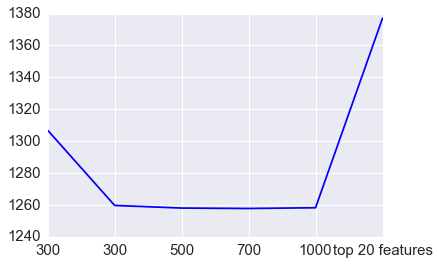
\includegraphics[width=0.5\textwidth]{rf_5models.png}
\end{tabular}}
\caption{Number of trees and Mean absolute error plot for Random Forest Regressors}
\end{figure}

\noindent
We could see that too many trees or not enough trees are both bad for prediction. Overall, the MAEs are above 1200, which is acceptable but not ideal. \\

\noindent
As for the Neural Network models, as I have explained in the ``Models'' Section, I could only try my best to focus on one aspect of the hyperparameters here in this task, I would like to see if a deeper network can be better than shallower networks or even Random Forest. Most of the time of this task is spent on this part and I am not showing the process of tuning neuron because it would be a little verbose and in the end I am not sure if this is the best set of number of neurons in every layer. Briefly speaking, my idea of such ``rough'' tuning is whether to decrease the number of neurons in every layer or first increase then decrease the number of neurons in every layer. I have also tried a couple of optimization metrics and I stopped trying once I get a relatively satisfying result (by comparing to the leaderboard). After setting these things up, I spend a lot of time tuning the depth of the network. In the Figure 4, I have mainly shown five models with more and more layers. \\

\begin{figure}[H]
\centerline{\begin{tabular}{cc}
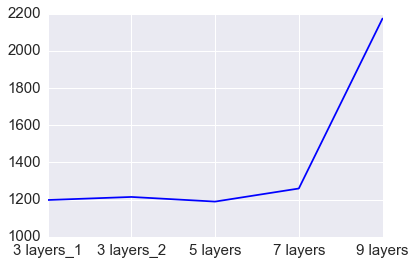
\includegraphics[width=0.5\textwidth]{nn_5models.png}
\end{tabular}}
\caption{Number of Layers and Mean Absolute Error plot for Neural Networks}
\end{figure}

\noindent
From the graph we can see that a deeper network with more layers is not necessarily better than a shallower network. While the numbers of neurons in the first two 3-layer cases show that there may not be significant difference in terms of small change in number of neurons in layers. The best model with the smallest MAE is the five-layer Neural Network, which is used for final prediction. \\


\noindent
5 Data Splits\\

\noindent
I have made up three data sets for split. One is the original data set with numerized categorical variables. It is split into $X_{train}, X_{test}, y_{train}, y_{test}$ with test size being one-third of the origin data rows. I have done the same thing for the scaled dataset and top principle component data set. \\

\noindent
Since the data is split in this way, we can do cross validation and make comparison between models. I would train my model on the same subset of the data so that the predictive accuracy on my test data sets can be used to compare among different models. Since I using mean-absolute-error as the metric, it would also be convenient to pick the best prediction to upload and compare with other teams. \\

\noindent
6 Errors and Mistakes\\

\noindent
The hardest part of the task is tuning the hyperparameters as the models I choose require a lot of computation. One model I have tried on but is not included in the report is the Gradient Boosting Random Forest. It took so long time to train a single model that it would be impossible to tune hyperparameters with my computer. The two models I choose here took much less time than GBRF but still can be very time-consuming. To tune the hyperparameter of Neural Network, I could only focus on one aspect (number of layers in this case) as the main hyperparameter to tune. Though I have tried various number of neurons in different layers and different optimization methods and some other hyperparameters to get the relatively best predicitons, I could not thoroughly go through each and every aspect of the hyperparameters of neural networks.\\

\noindent
7 Predictive Accuracy\\

\noindent
Username:\verb| yz273_Darien Zhang|\\

\noindent
From the mean-absolute-error values of the models I have tried, we can conclude that Neural Networks perform better than Random Forest Regressors. Within the Neural Networks, it is not necessarily true that deeper structure works better. A comparision of effectiveness among the models via mean-absolute-error can be seen in Figure 3 and 4.  The best network I have tried is a five-layer network. Here I have attached the graphs of the true values and predictions of the best model for displaying the accuracy.  

\begin{figure}[H]
\centerline{\begin{tabular}{cc}
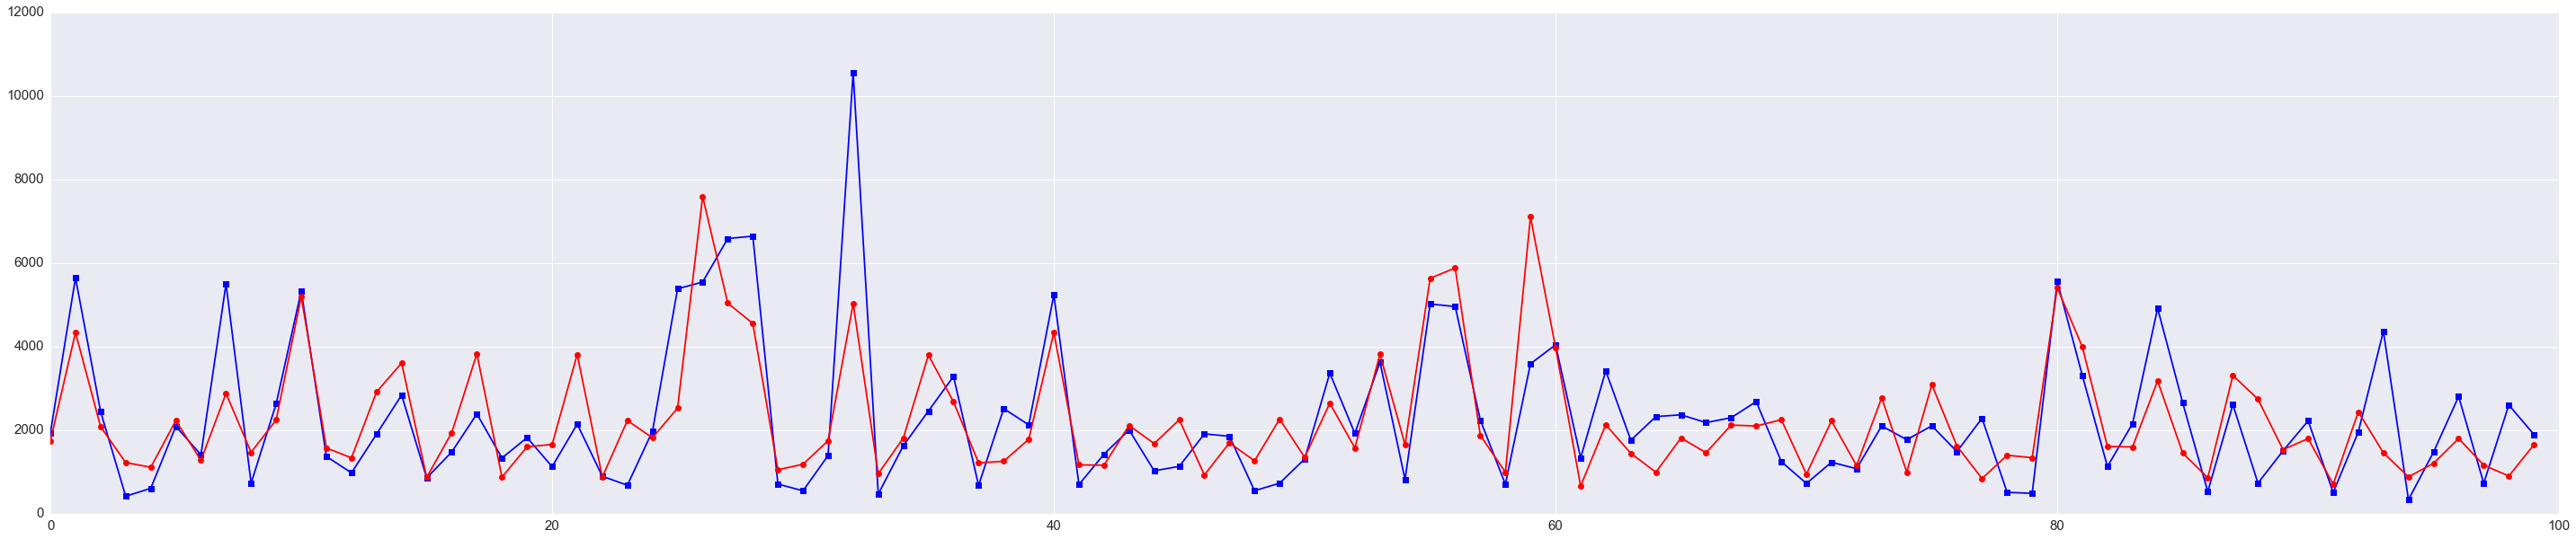
\includegraphics[width=0.5\textwidth]{first100_pred.png}
\end{tabular}}
\caption{First 100 predictions and true values (Red points are predictions)}
\end{figure}

\begin{figure}[H]
\centerline{\begin{tabular}{cc}
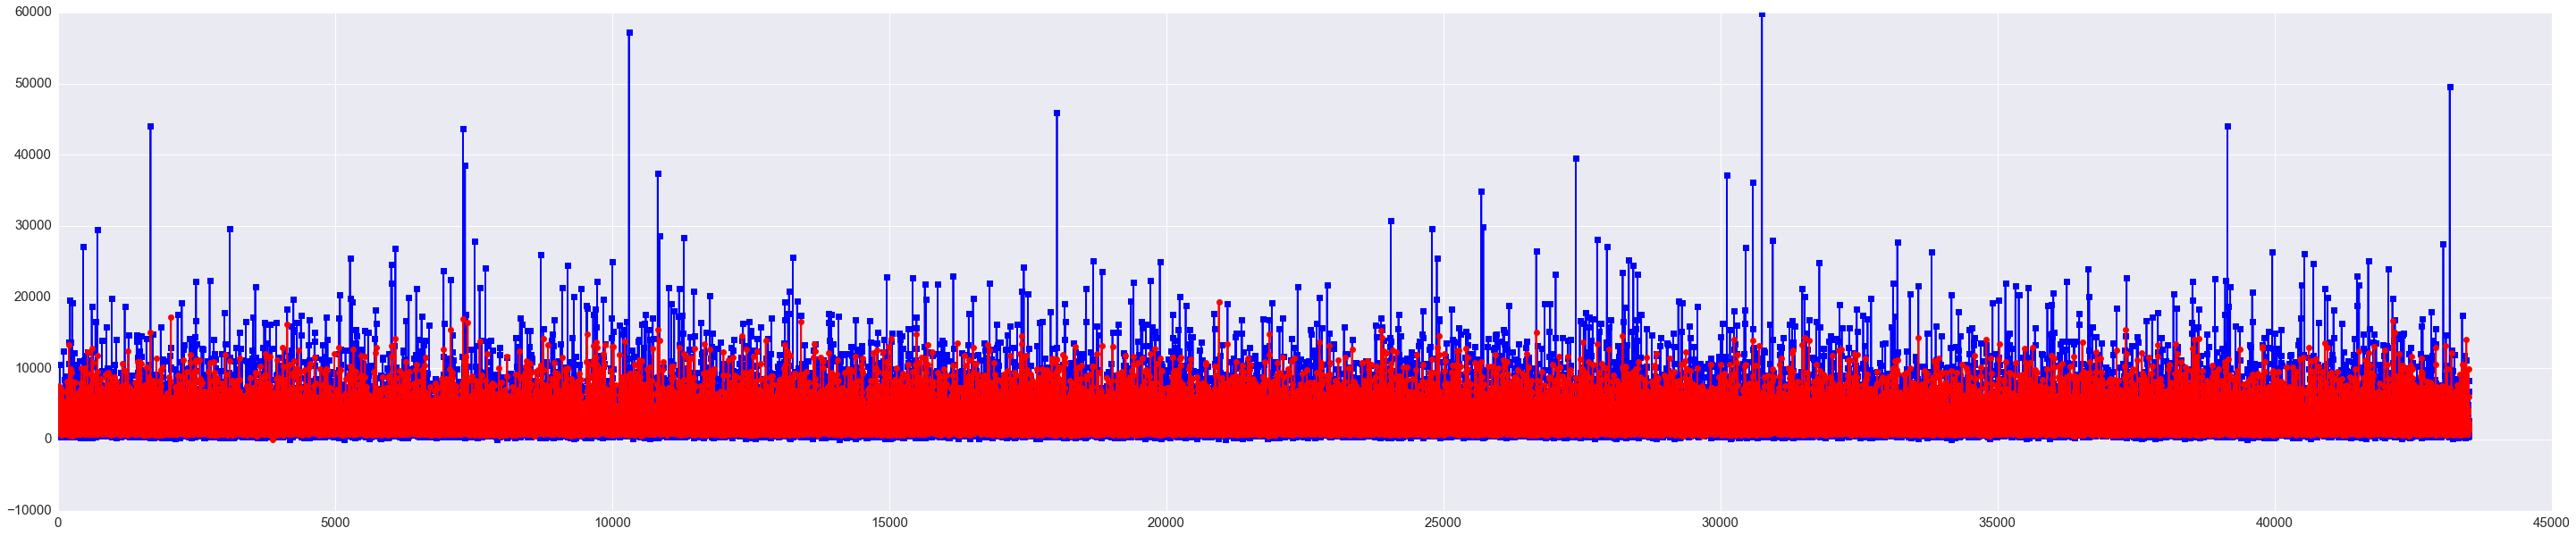
\includegraphics[width=0.5\textwidth]{all_pred.png}
\end{tabular}}
\caption{All predictions and true values (Red points are predictions)}
\end{figure}

\noindent
From the graphs we can see that the prediction catches the pattern pretty nicely, while the exact predictions on some big values are not ideal, which causes an increase in the MAE.\\

\noindent
8 Code \\
(attached with output from ipython notebook)
\end{document}
